%! Author = Saeid Yazdani
%! Date = 4/1/2024


\section{Load Board Evaluation}
\label{sec:loadboard-evaluation}

To rule out load board issues, the load board needs to be
tested out of circuit.
Measurements such as impedance, capacitance, and propagation delay of traces
connecting \ac{ATE} test head to the \ac{DUT} will give a better insight into
localizing error sources.

The load board is based on a multi-layer PCB, and power planes give us low
impedance between ATE pogo pins and socket pogo pins.
In the following, we will summarize the findings on the power plane and signal
trace measurements.

\subsection{Basic Load Board Design Rules}
\label{basic-load-board-design-rules}

The quality of a load board to interface a \ac{DUT} to an \ac{ATE} is
essential for precise testing.
The advent of high-speed devices, such as \ac{LVDS} and \ac{TDMS} imposes
stringent performance demands on \acp{ATE}, particularly concerning
load boards \autocite{1041807}.

There are well-defined design rules for all signal and power traces.
the following list summarizes some of the important rules that a
well-designed load board needs to obey:
% Interfacing, often a performance bottleneck between ATE and device under test

\begin{itemize}[topsep=8pt,itemsep=4pt,partopsep=4pt, parsep=4pt]

    \item Constant impedance of traces \autocite{36225}
    \begin{itemize}
        \item \SI{50}{\ohm} impedance on almost all traces are expected unless
        otherwise noted signal traces such as utility traces, sense lines,
        etc.

        \item Impedance shall stay between \SI{49}{\ohm} and \SI{51}{\ohm}.
    \end{itemize}

    \item Timing differences between signals should ideally not exist

    \item Use sufficient space between traces and drill holes

    \item Use \ac{HT} FR4 material to withstand temperature tests.

    \item In case of using support components such as decoupling capacitors,
    multiplexers, shift registers, relays, etc. on a load board, the
    temperature and current rating of all components must be compliant with
    the maximum test temperature.
    \begin{itemize}
        \item If not possible, such components must be placed far away from
        \ac{DUT} socket to avoid contact with the \emph{thermal head}
        (\autoref{fig:thermal-head-on-ate})
    \end{itemize}

    \item All \ac{DGS} lines of the \ac{ATE}'s
    \ac{DPS} units must be connected to the ground plane on the load board
    to ensure correct control loop behavior of \ac{DPS} units
    \begin{itemize}
        \item Valid for all comparator's \ac{DGS} ground sense, channel
        card \ac{DGS}, and calibration \ac{DGS} lines

        \item \emph{Measure Return} should be connected to the ground plane
        \item \ac{DGS} must be connected to the ground plane
    \end{itemize}

    \item \ac{DGS} must be connected to the ground plane close to the
    \ac{ATE} pogo pin
    \item Power sense lines must be connected to power as close to the
    \ac{DUT} socket as possible
    \item Ground loops must be avoided
    \item For analog peripherals that require low noise for testing,
    shielding with ground planes is necessary

\end{itemize}

\subsection{Load Board Measurement Setup}
\label{loadbaord-measurement-setup}

In low-level measurements, the stability of a measurement setup is crucial, as
any vibration can translate into noise and distort the
measurement results due to piezoelectric and microphonic effects.

Therefore, for performing sensitive measurements on the load board, the
load board is bolted to a test stand with a set of four individually adjustable
pogo arms that can be placed everywhere on the load board as shown in
\autoref{fig:villach-loadboard-measurement-setup}.
The pogo pins for making contact with the copper pads on the load board are
wired using low-leakage shielded coaxial cables.

\begin{figure}[htbp]
    \centering
    \printfitgraphics[0.62\textheight]{figures/villach-supply-analysis/loadboard/mes-setup/loadboard-measurement-stand}
    \caption[Load Board Measurement Setup]{
        Measurement setup for evaluating the load board.
        Top: Front side of the load board where four \acs{DUT} sites are visible
        which one site is populated with a test socket.
        Bottom: The back side of the load board where contact to \ac{ATE}'s
        test head is located.
    }
    \label{fig:villach-loadboard-measurement-setup}
\end{figure}

\subsection{Load Board Measurement Results}
\label{loadbaord-measurement-results}

The load board contains four \ac{DUT} sites.
Three of the sockets were removed so that the
measurements contain purely a dataset of the load board itself (the sockets
were evaluated separately).

From each of the \ac{DUT} sites, 50 signal traces were chosen for the
measurements.
Before performing measurements, the following information was taken
from the \ac{PCB} layout \ac{CAD} tool:

\begin{itemize}[topsep=8pt,itemsep=4pt,partopsep=4pt, parsep=4pt]
    \item \textbf{Trace length:} The length of the traces from the \ac{ATE}'s
    test head contact point to the copper pad of the \ac{DUT} socket
    \item \textbf{Trace width:} The width of the traces
\end{itemize}

The following findings were concluded:

\begin{itemize}[topsep=8pt,itemsep=4pt,partopsep=4pt, parsep=4pt]

    \item \ac{TDR} data show gross deviations between trace delays and the
    maximum tolerable delay variations near limit.
    The board is not an equal-length design and tester signals
    arrive at different instances of time at the DUT.

    \item Signal traces are not terminated, and trace lengths vary drastically
    between all \ac{DUT} sites.
    Hence, the layout design is targeted towards low speed.
    Gross varying delay times dictate that test speed must be kept low in order
    not to introduce timing problems during the test, or the timing of each signal
    line must be adapted and corrected.

\end{itemize}

In an \ac{ATE} environment, the ideal scenario for load boards is to have all
signal traces for all \ac{DUT} sites equal in length as
this simplifies the test program development and ensures equal response to test
events in case of Multi-\ac{DUT} load boards.

Trace length influences signal integrity.
Signal attenuation and rise time degradation
can occur which can lead to incorrect readings of digital levels
in high-speed digital \acp{DUT}.
Length matching is always mandatory for high-speed data signals such
as \ac{USB} and \ac{LVDS} which rely on differential pairs.

In addition to signal integrity issues, longer traces can lead to \ac{EMC}
related issues simply because a long trace can act as an antenna,
emitting or receiving \ac{EMI} which may affect overall test results.

Other issues such as voltage drop and power integrity may arise if long traces
are part of \acp{PDN}.
The load board under investigation has multiple large power planes dedicated
to the main supply line and there are no long traces for these supply lines as
the power traces are directly coming out of power planes and connect to \ac{DUT}
copper pads in a relatively short length.

\subsection{Power Plane Capacitances}
\label{subsec:loadboard-powerplane-capacitances}

The power planes of a \ac{PCB} can hold an electrical charge and therefore
act as a capacitor.
This inter-plane capacitance, while not large when compared to discrete
decoupling capacitors (typically \SI{10}{\nano\farad} to \SI{10}{\micro\farad}),
can be exploited to form embedded capacitors within
\ac{PCB} layers \autocite{7810044}.

At \SI{60}{\centi\meter} by \SI{40}{\centi\meter}, the load board under
investigation is relatively large compared to a typical
\ac{PCB} and therefore any capacitance resulting from power planes will be part
of decoupling scheme.

Since the load board is populated with multiple support components, it is not
possible to measure the capacitance of the power planes individually.
Using \autoref{eq:power-plane-capacitance}, theoretical power plane
capacitance of the load board with dedicated layers for a given supply rail
can be estimated.

Assuming standard FR4 material (dielectric constant around
\SI{4.4}) and a layer stack distance of \SI{0.2}{\milli\meter}
the resulting inter-plane capacitance will be
approximately \SI{50}{\nano\farad}.
Although this amount is relatively small, it still contributes to the overall
start-up stability of the \ac{DPS} units.

\begin{equation}
    \label{eq:power-plane-capacitance}
    C = \frac{\varepsilon_r \cdot \varepsilon_0 \cdot A}{d}
\end{equation}

Further investigations reveal that there are power planes assigned to each of
the major voltage rails that are required by the \acp{DUT}.
For example, the \SI{1.3}{\volt} or $V_{DD}$ plane for all
of the four \ac{DUT} sites is located on the second layer and there is a ground
plane directly placed on the third layer.
This $V_{DD}$ planes are isolated per \ac{DUT} site, meaning that each \ac{DUT}
should be powered up with a separate \ac{DPS} unit.

Furthermore, each $V_{DD}$ plane has a unique geometry and therefore a different
contribution to the total capacitance as seen from the assigned power source
as well as different decoupling properties for \ac{RF} decoupling,
as shown in \autoref{fig:villach-loadboard-1v3_GND_planes}.
The other voltage rails follow the same design: asymmetric planes within some
inner layers are assigned to these rails and each of these layers is followed
by a complete layer assigned to ground (reference) plane.

\begin{figure}[htbp]
    \centering
    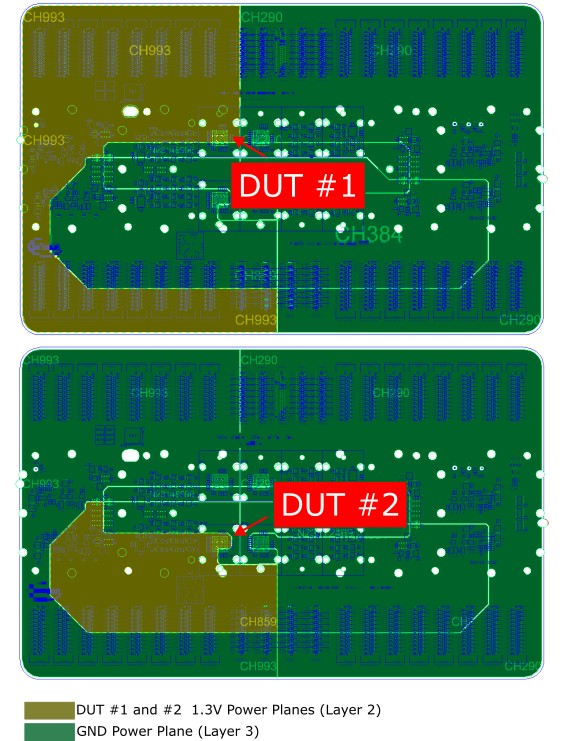
\includegraphics[width=\linewidth,height=0.62\textheight,keepaspectratio,interpolate=false]
    {figures/villach-supply-analysis/loadboard/groun-planes-example_1v3_GND.jpg}
    \caption[\acs{DUT} \#2 \emph{VDD} and \emph{GND} power planes]{
        Power plane layout of \SI{1.3}{\volt} rail and its immediate ground
        layer (Top: \ac{DUT} site \#1, Bottom: \ac{DUT} site \#2).
        The geometries of these power planes are not symmetrical.
    }
    \label{fig:villach-loadboard-1v3_GND_planes}
\end{figure}








